%
%   $Id$
%   This file is part of the FPC documentation.
%   Copyright (C) 2000 by Florian Klaempfl
%
%   The FPC documentation is free text; you can redistribute it and/or
%   modify it under the terms of the GNU Library General Public License as
%   published by the Free Software Foundation; either version 2 of the
%   License, or (at your option) any later version.
%
%   The FPC Documentation is distributed in the hope that it will be useful,
%   but WITHOUT ANY WARRANTY; without even the implied warranty of
%   MERCHANTABILITY or FITNESS FOR A PARTICULAR PURPOSE.  See the GNU
%   Library General Public License for more details.
%
%   You should have received a copy of the GNU Library General Public
%   License along with the FPC documentation; see the file COPYING.LIB.  If not,
%   write to the Free Software Foundation, Inc., 59 Temple Place - Suite 330,
%   Boston, MA 02111-1307, USA.
%
%%%%%%%%%%%%%%%%%%%%%%%%%%%%%%%%%%%%%%%%%%%%%%%%%%%%%%%%%%%%%%%%%%%%%
% Using the IDE
%%%%%%%%%%%%%%%%%%%%%%%%%%%%%%%%%%%%%%%%%%%%%%%%%%%%%%%%%%%%%%%%%%%%%
\chapter{Using the IDE}

The IDE (\textbf{I}ntegrated \textbf{D}evelopment \textbf{E}nvironment)
provides a comfortable user interface to the compiler. Moreover, it
provides a debugger, symbol browser etc. The IDE is a textmode
application which allows the same look and feel for all supported
operating systems. Furthermore, it will be very familiar to all
Turbo Pascal users.
Currently the IDE is available for DOS, Win32 and Linux.

\section{First steps with the IDE}

The IDE is started by entering the command:
\begin{verbatim}
fp
\end{verbatim}
at the command line. Of course, you can also start the IDE
from a graphical user interface (under the Windows enviroment, you
can switch between windowed mode and full screen mode by pressing
\textsc{Alt-Enter}).

\subsection{The IDE screen}

\begin{htmlonly}
After start up, the screen of the IDE looks like this:
\htmladdimg{../pics/idestart.gif}
\end{htmlonly}
\begin{latexonly}
After start up, the screen of the IDE looks like figure \ref{fig:idestart}.
\begin{figure}
\caption{The IDE screen immediatly after startup}
\label{fig:idestart}
\ifpdf
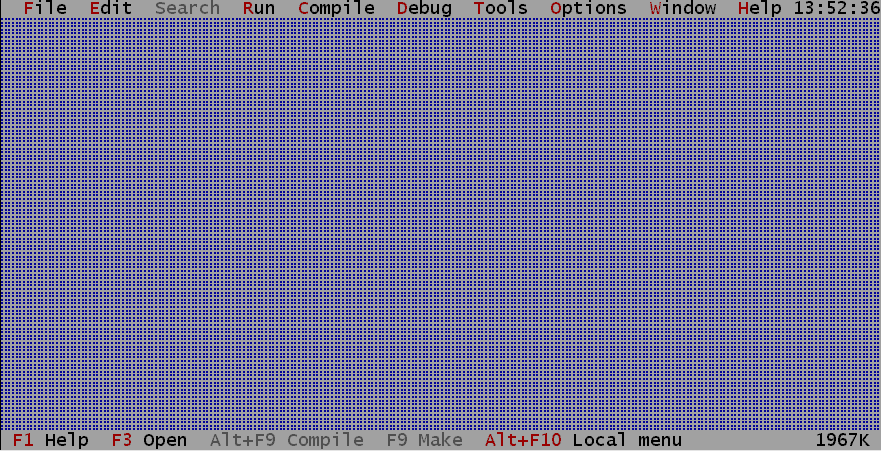
\epsfig{file=pics/idestart.pdf,width=\textwidth}
\else
%%%%%%%%%% !!!!!!!! eps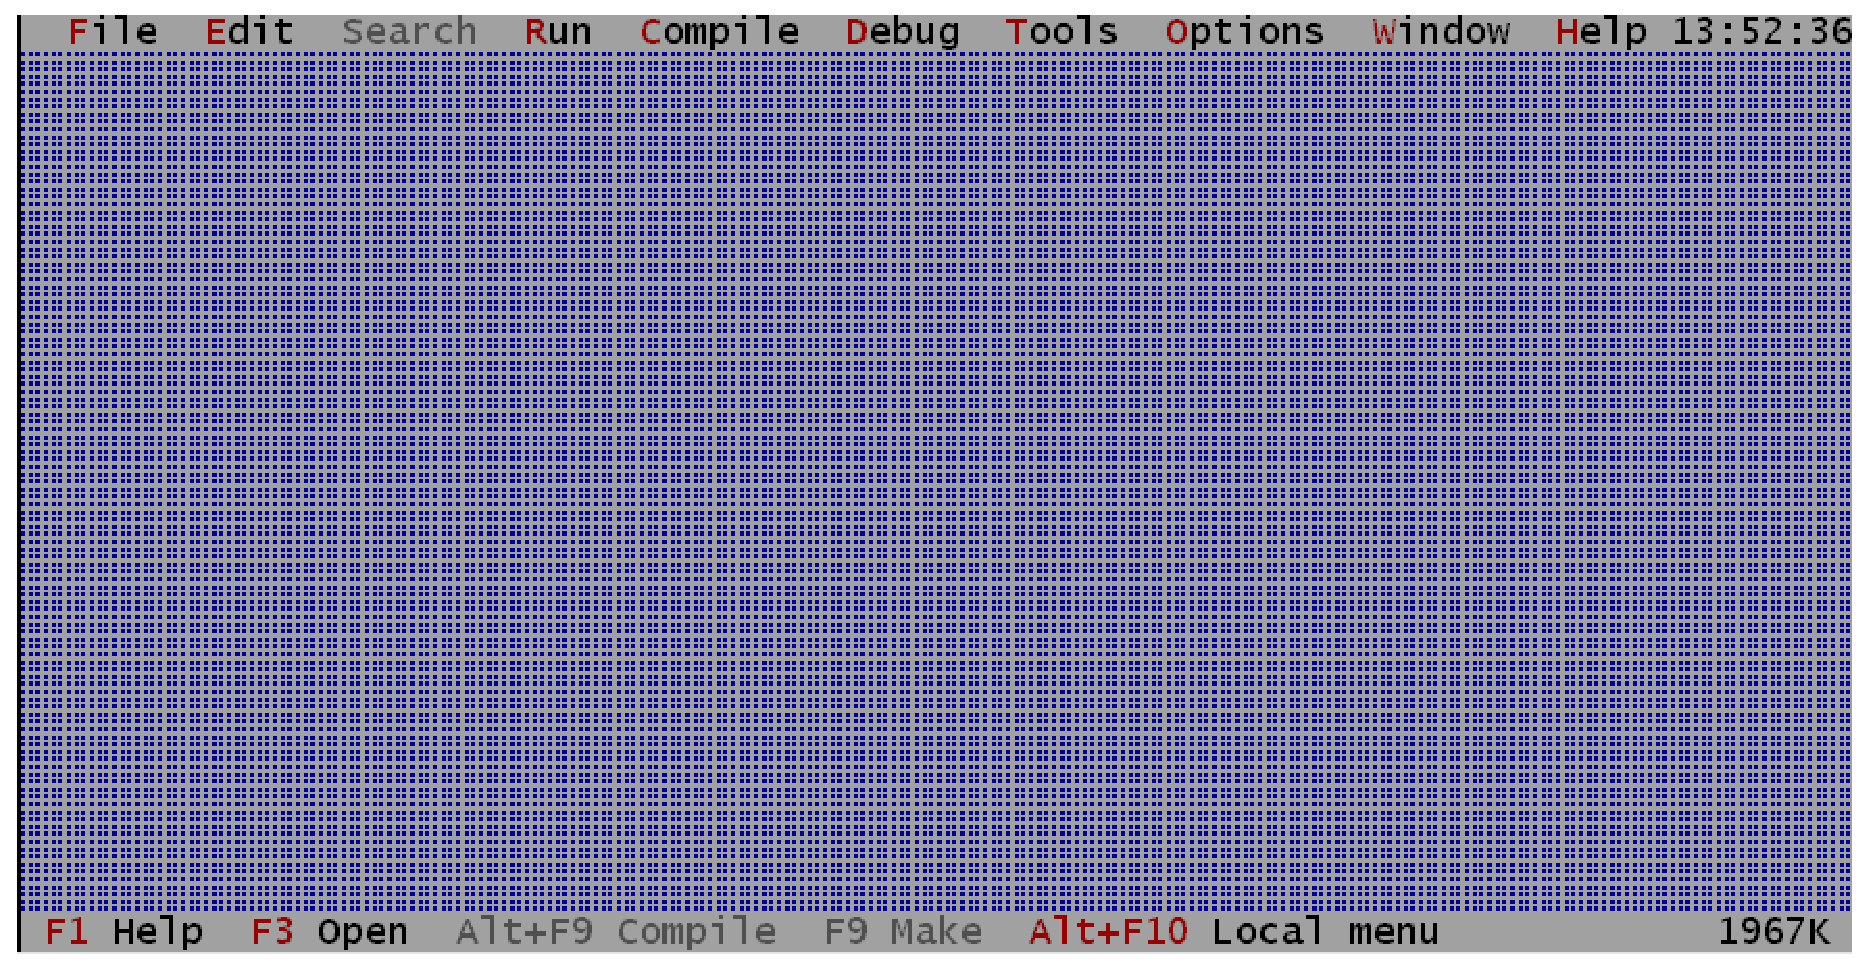
\epsfig{file=pics/idestart.eps,width=\textwidth}
\fi
\end{figure}
\end{latexonly}
At top of the screen you see the \emph{menu bar}, at the bottom
the \emph{status bar}. The empty bar between them is called the
\emph{desktop}.

The statusbar allows a quick access to often used commands by
clicking them with the mouse. Further, it reminds you about 
keyboard shortcuts that are frequently used.

In upper right corner of the IDE screen a clock is displayed to
remind you to go to bed in time. At lower right corner you'll
see the current amount of unsed memory. Don't worry if this value
is low - the IDE allocates more memory from the operating system
if it runs out of memory.

You can exit from the IDE by selecting \var{File|Exit}
\footnote{\var{File|Exit} means select the item Exit in the menu File}
or by pressing \textsc{Alt-X}.

\begin{remark}
A complete reference of all keyboard shortcuts can be found in
section \ref{ide:keyshortcuts}.
\end{remark}

\subsection{IDE Command line options}

When starting the IDE, command line options can be passed:
\begin{verbatim}
fp [-option] [-option] ... <file name> ...
\end{verbatim}

\var{Option} is one of the following switches (the option letters
aren't case sensitive):

\begin{description}
\item [-N] DOS only: Do not use long file names. Since Windows 95 an interface
is provided to DOS applications to access long file names. The IDE uses
this interface by default to access files. Under certain circumstances, this
can lead to problems.
\item [-Cfilename] This option followed by
a filename uses the given file to read the options. The file name
must follow the \var{C-} without spaces.
\item [-R] After starting the IDE, it changes automatically to the directory
which was active when you left the IDE the last time.
\end{description}

The files given at the command line are loaded into edit
window automatically.

\begin{remark}
Under DOS/Win32, \var{/} can be used instead of \var{-} to pass a
command line switch to the IDE.
\end{remark}

\subsection{Using the mouse}
\label{ide:mouseusage}
If the system is equipped with a mouse, it can be used to work with the
IDE. The left button is used to select menu items, press buttons, select
text blocks etc. The right mouse button is used to access the local menu.
The local menu isn't always available. Holding down the \textsc{Ctrl} or
\textsc{Alt} key and clicking the right button will
execute user defined functions, see \ref{ide:prefmouse}

\begin{remark}
Occasionally, this manual uses the term "drag the mouse". This
means that you have to move the mouse while pressing the left
mouse button.
\end{remark}

\begin{remark}
When talking about left and right mouse button, it always means that the
mouse buttons aren't reversed, if you want you can exchange the
behavior of the left and right mouse button, see \ref{ide:prefmouse}.
\end{remark}

\begin{remark}
Under the following circumstances you won't be able to use the mouse,
even if your system has one:
\begin{itemize}
\item The IDE is running under Linux throught a telnet connection
\item The IDE is running under Linux in a window
\end{itemize}
\end{remark}

\subsection{Accessing the menu}
The menu (the gray bar at the top of the IDE) can be accessed by using
the mouse to select items. If you do not use a mouse, you can use
\textsc{F10} to switch to the menu. Use the arrow keys to navigate
and the \textsc{Enter} key to select items.
To access the menu very fast without leaving the
keyboard with your hands, \textsc{Alt-<highlighted letter>}
can be used, afterwards
menu entries can be selected by pressing also the highlighted letter, but
without \textsc{Alt}. E.g. \textsc{Alt-S G} is a fast way to
display the \emph{goto line dialog}.

Every menu item is explained by a short text in the status bar.

In certain cases, a local menu is available. It can be accessed by pressing
the right mouse button or \textsc{Alt-F10}.

%%%%%%%%%%%%%%%%%%%%%%%%%%%%%%%%%%%%%%%%%%%%%%%%%%%%%%%%%%%%%%%%%%%%%%%
% Windows
\section{Windows}
In our days, working with windowed applications should be familiar to
most users. Nevertheless, the following section describes how
the windows work in the \fpc IDE to allow an efficient work with it.

\subsection{Basics}
\begin{htmlonly}
A common IDE window looks like:
\htmladdimg{../pics/idewin.gif}
\end{htmlonly}
\begin{latexonly}
Figure \ref{fig:idewin} shows a common IDE edit window.
\begin{figure}
\caption{A common IDE window}
\label{fig:idewin}
\ifpdf
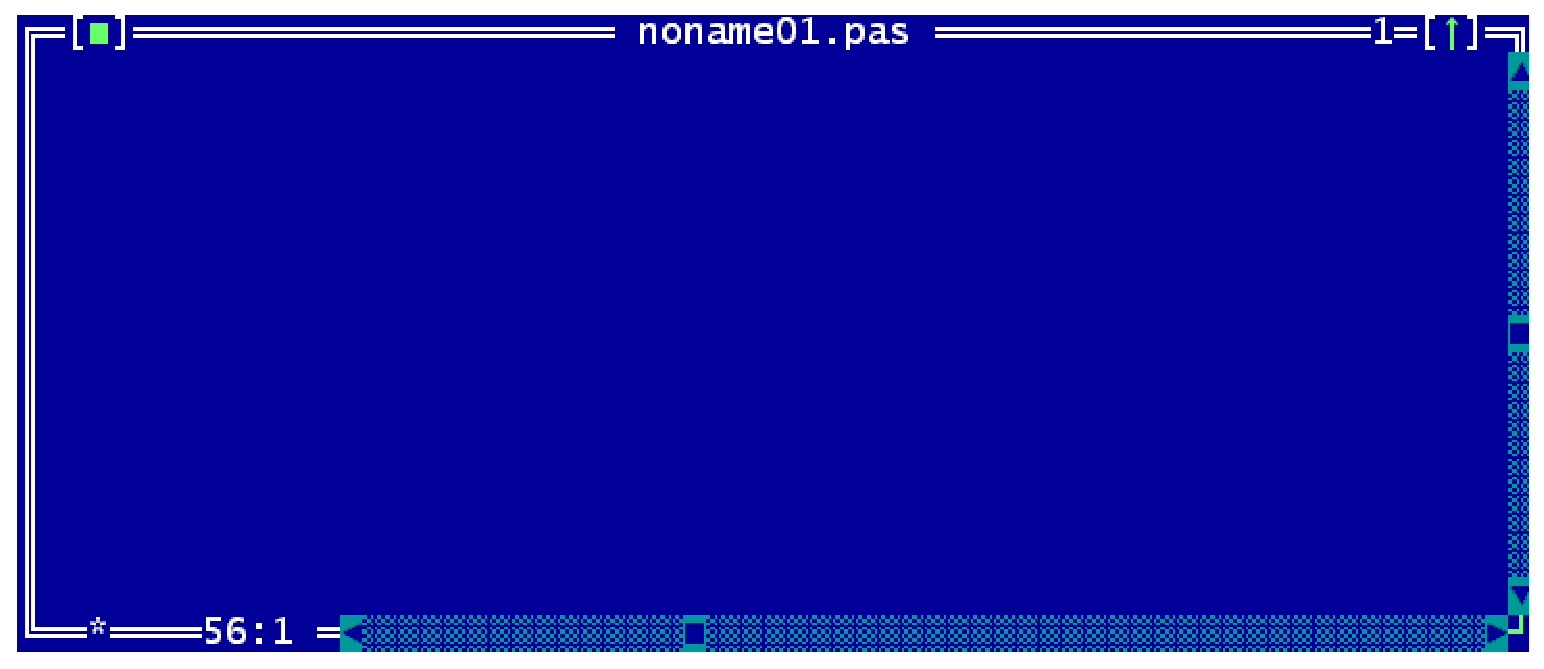
\epsfig{file=pics/idewin.pdf,width=\textwidth}
\else
%%%%%%%%%% !!!!!!!!eps 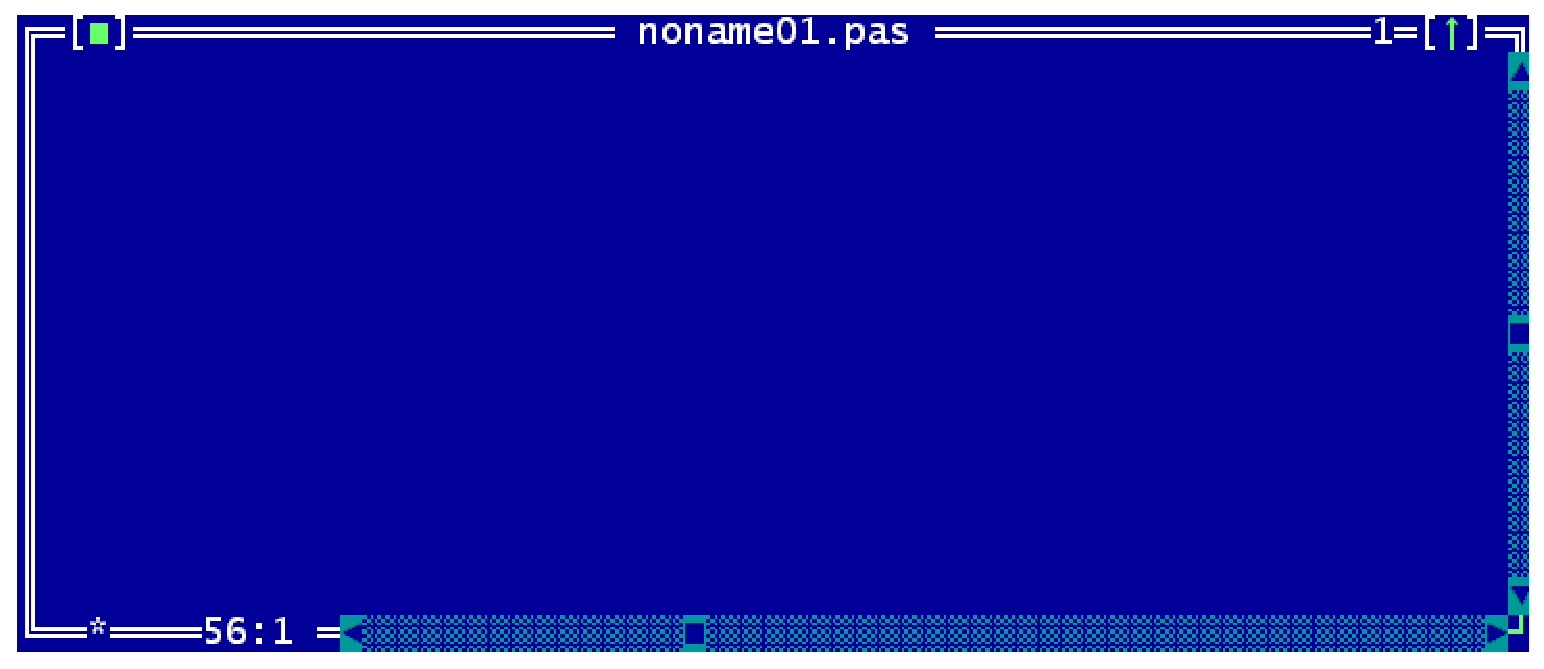
\epsfig{file=pics/idewin.eps,width=\textwidth}
\fi
\end{figure}
\end{latexonly}
The window is surround by the so called \emph{frame}, the whith double
line around the window.
At the top of the window you'll see the title bar, it contains the title
of the window (what else?). To move the window click, on
the title bar and drag the window with the mouse.
If you do not have a mouse, see \ref{ide:keyboardwindow} how
to use the keyboard to work with windows.

At the upper left corner you see the \emph{close icon}. If you click it the
window will be closed, it can be also closed by pressing \textsc{Alt-F3} or
selecting the menu item \var{Window|Close}. All open windows can be closed
by selecting the menu item \var{Window|Close all}.

To resize the window, click on the lower left corner of the window
and drag it (move the mouse while holding the left button pressed).
Keyboard users should look at section \ref{ide:keyboardwindow}.
Not all windows can be resized. This applies, for example, to
\emph{dialog windows} (\ref{ide:dialogwindow}).

At the upper right you'll see a green arrow. Clicking this arrow
zooms the window to the whole desktop. If you click this arrow on
a zoomed window, the old size of the window will be restored. Pressing
the key \textsc{F5} has the same effect as clicking that arrow. Furthermore,
this can be also done by selecting the menu item \var{Window|Zoom}.
Windows which aren't resizeable can't be zoomed, either.

The scrollbars at the right and bottom border can be used to scroll
the window contents with the mouse. Click on the arrows to scroll
line by line and on the dotted area between the arrows and the
cyan-coloured
rectangle to scroll page by page. By dragging the rectangle you can
scroll continously through the window contents.

The star and the numbers in the lower left corner
are explained in the section about the editor, see \ref{ide:editingtext}.

\subsection{Working with multiple windows}
When working with larger projects, you'll have multible windows on your
desktop. An inactive window is identified by a grey frame. You can
activate it by clicking on the window with the mouse. Or you can
step trough all open windows by pressing \textsc{F6}
(menu item \var{Window|Next}).
To activate the last activated window, press \textsc{Shift-F6}
(menu item \var{Window|Previous}).

If the window has a number in the upper
right corner, you can activate it by pressing \textsc{Alt-<number>}.
\textsc{Alt-0} has a special meaning,
it shows a dialog box with all available
windows which allows a quick activation of windows which don't have a
number.

Of course, you can order the windows on the IDE desktop by zooming and
resizing them with the mouse or keyboard. This is particularly difficult
with the keyboard. Instead, you can use the menu items
\var{Window|Tile} and \var{Window|Cascade}. Tile means that the
whole desktop space is divided up evenly between all resizable
windows. \emph{Cascade} brings
all windows in a cascaded position. Just try these commands if you've
multiple windows on the IDE desktop.

In very rare cases the screen of the IDE may be mixed up. In this
case the whole IDE screen can bebe refreshed by selecting
the menu item \var{Window|Refresh display}.

\subsection{Dialog windows}
\label{ide:dialogwindow}
In many cases the IDE displays a dialog window to get user input.
The main difference to other windows is that you can't activate
other windows while a dialog is active. This behavior is called
\emph{modal}. To activate another window, you've to close
a modal window/dialog.

\begin{htmlonly}
A typical dialog window looks like:
\htmladdimg{../pics/idedlg.gif}
\end{htmlonly}
\begin{latexonly}
Figure \ref{fig:idedlg} shows a typical dialog window.
\begin{figure}
\caption{A typical dialog window}
\label{fig:idedlg}
\ifpdf
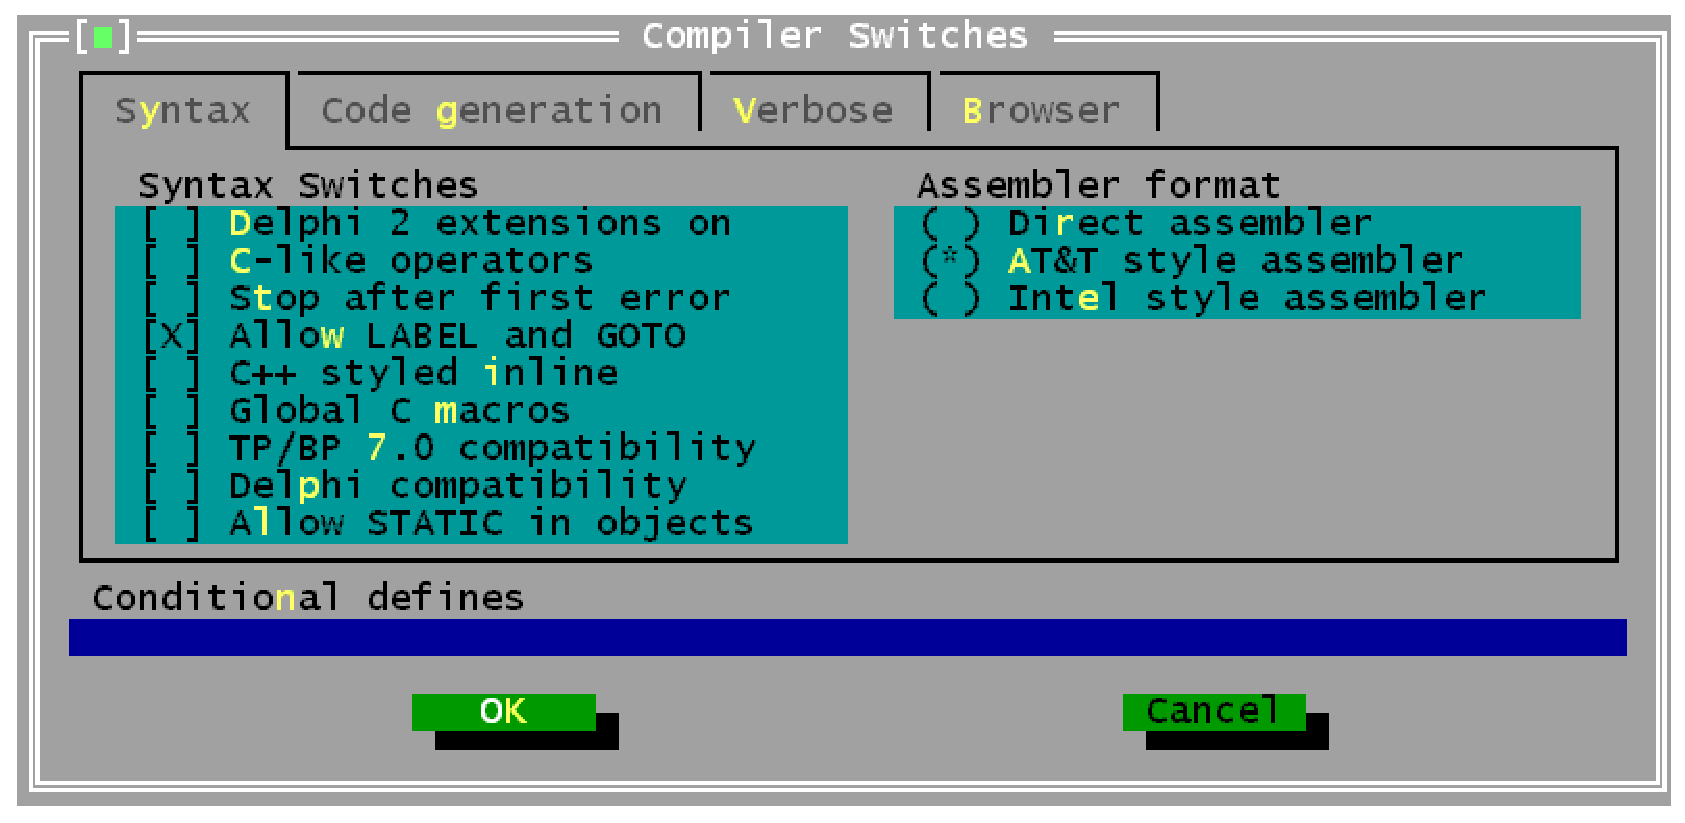
\epsfig{file=pics/idedlg.pdf,width=\textwidth}
\else
%%%%%%%%%% !!!!!!!!eps 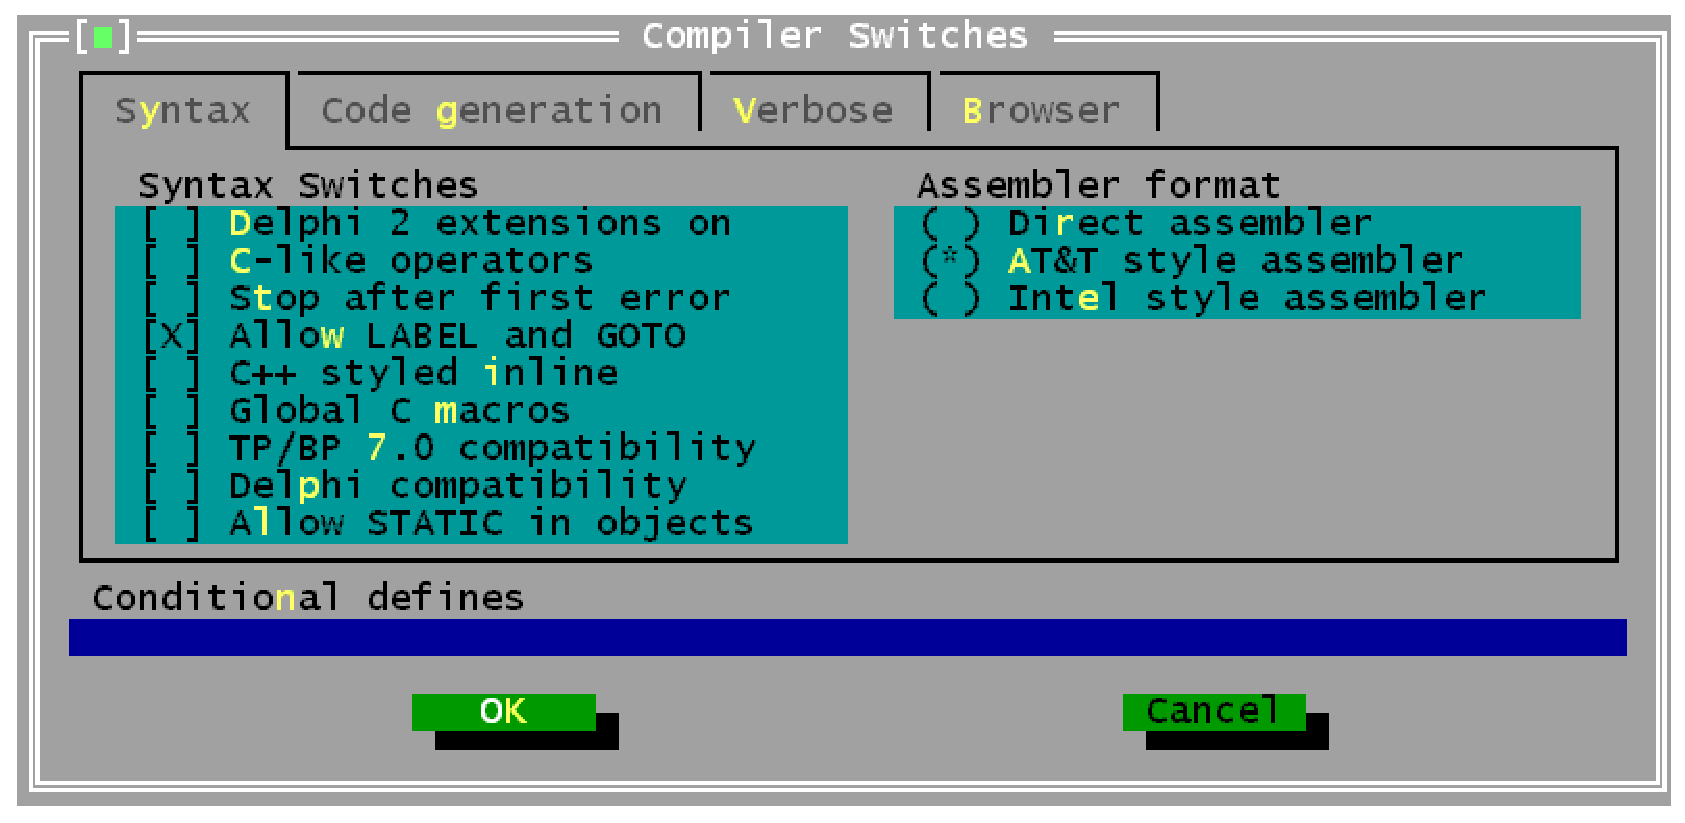
\epsfig{file=pics/idedlg.eps,width=\textwidth}
\fi
\end{figure}
\end{latexonly}
%%%!!!!!!!!!!!!!!

\subsection{Moving and zooming windows with the keyboard}
\label{ide:keyboardwindow}
To resize/move a window with the keyboard, go into the size/move mode
by pressing \textsc{Ctrl-F5} or selecting the menu item
\var{Window|Size/Move}. Now the window frame will be green. Using the
cursor keys you can move the window. By pressing shift and the cursor
keys, the window can be resized. The size/move mode can be left by pressing
\textsc{Enter}. In this the window will keep it's size and position.
Alternativly, you can press \textsc{Esc} and the old size will be restored.

%%%%%%%%%%%%%%%%%%%%%%%%%%%%%%%%%%%%%%%%%%%%%%%%%%%%%%%%%%%%%%%%%%%%%%%
% The help system
\section{The help system}
If you are stuck somewhere while editing files, regarding the syntax
of a pascal statment or the behavior of a subroutine of the runtime
library, you can use the \emph{help system} to get some information. The
help system is called up by pressing F1.

\subsection{Navigating in the help system}
The help system contains hyperlinks which can be accessed by clicking
them with the mouse. Alternativly, \textsc{Tab} and \textsc{Shift-Tab}
can be used to move between the different hyperlinks of a page
and the \textsc{Enter} key can be used to select them.

The contents of the help system is displayed, if you press \textsc{Shift-F1}.
To go back to the last help topic, \textsc{press Alt-F1}. This also works
if the help window isn't displayed on the desktop.

\subsection{Working with help files}
The IDE contains a help system which can display HTML files
as well as the TPH format known from TP. Of course, the HTML
viewer of the help system is limited, so forget about displaying
HTML files which use e.g. CSS \footnote{\textbf{C}ascaded
\textbf{S}tyle \textbf{S}heets, an extension to HTML to
get a similiar look like of a document with all browsers}. It is designed to display the FPC
help files, but feel free to improve it and send us patches...

The menu item \var{Help|Files} permits you to add and delete
help files.

Press the \emph{new button} to add a new file. You'll be asked to enter
the location of the help file. If it is an
HTML file, a dialog box will be displayed
which asks for a title. This title will then be included in the
contents of help.

A help file can be deleted from the help system (it ISN'T deleted from
your hard disk) by pressing the \emph{delete button}.

\subsection{The about dialog}
The \emph{about dialog} (\var{Help|About...}) shows some information
about the IDE, please include versions and dates of this
dialog if you report bugs, have suggestion etc regarding the IDE.
Furthermore, it contains copyright information.

%%%%%%%%%%%%%%%%%%%%%%%%%%%%%%%%%%%%%%%%%%%%%%%%%%%%%%%%%%%%%%%%%%%%%%%
% Editing text
\section{Editing text}
\label{ide:editingtext}
%%%!!!!!!!!!!!!!!

\subsection{Insertion modes}
%%%!!!!!!!!!!!!!!

\subsection{Setting marks}
The IDE provides a feature which permits you to set a mark at
the current cursor position. Later, you can return to this
position by pressing a keyboard shortcut.

You can set up to 9 marks per source file, they are set by
\textsc{Ctrl-K-<Number>} (where number is the number of the mark).
To go to a previous set mark, press \textsc{Ctrl-Q-<Number}.

\begin{remark}
Currently, the marks aren't stored if the IDE is left. This may
change in future implementations of the IDE.
\end{remark}

%%%%%%%%%%%%%%%%%%%%%%%%%%%%%%%%%%%%%%%%%%%%%%%%%%%%%%%%%%%%%%%%%%%%%%%
% Searching in the text
\section{Searching in the text}
\label{ide:searching}


\subsection{The symbol browser}
%%%!!!!!!!!!!!!!!

%%%%%%%%%%%%%%%%%%%%%%%%%%%%%%%%%%%%%%%%%%%%%%%%%%%%%%%%%%%%%%%%%%%%%%%
% Running programs
\section{Running programs}
\label{ide:running}
%%%!!!!!!!!!!!!!!

%%%%%%%%%%%%%%%%%%%%%%%%%%%%%%%%%%%%%%%%%%%%%%%%%%%%%%%%%%%%%%%%%%%%%%%
% Debugging programs
\section{Debugging programs}
%%%!!!!!!!!!!!!!!

%%%%%%%%%%%%%%%%%%%%%%%%%%%%%%%%%%%%%%%%%%%%%%%%%%%%%%%%%%%%%%%%%%%%%%%
% The tools menu
\section{The tools menu}
\label{ide:toolsmenu}
The tools menu allows you an easy access to external tools. Further,
it contains two other probaly helpful tools for programmers: an
ascii table and a calculator.

\subsection{The messages window}
The output of the external utilies is redirected by the IDE and it
will be displayed in the message window. The message window is
displayed automatically, if an external tool was run. The
messages window can be also display manual by the selecting the
menu item \var{Tools|Messages} or by pressing the key \textsc{F11}.

If the output of the tools contains filenames and line numbers,
you can goto the source line by pressing \textsc{Enter} or
double clicking the output line. To trace the source, press
\textsc{Space}. The difference between goto and tracking is that
goto closes the message window while tracking keeps the message
window active and the source file is displayed only in the background.

The algorithm which extracts the file names and line numbers from
the tool output is quite sophisticated, but in some cases it may
fail. In this case, please refer the sources of the IDE.

\subsection{GREP}
One external tool in the Tools menu is already predefined: an
menu item to call the \file{grep} utility (\var{Tools|Grep} or
\textsc{Shift-F2}). \file{grep} search for a given string in files and
returns the lines which contain the string. The search string can
be even a regular expression (see \ref{ide:regexpr}).

\subsection{The ascii table}
The tools menu provides also an ascii table (\var{Tools|Ascii table},
it allows you to lookup ascii codes as well as
inserting chars into the window which was active when calling the
ascii chart. To get the ascii code of a char move the blocking block
cursor on this char or click with the mouse on it. To insert a
char into an editor window, double click it with the mouse
or press \textsc{Enter} while the cursor is on it.

\subsection{The calculator}
The calculator allows you to do quickly some calculations. It doesn't
take care of operator precedence, so be careful. For more information
about the supported operations, see table \ref{ide:calculatorcommands}.

\begin{FPCltable}{p{5cm}lll}{Calculator commands}{calculatorcommands}
\label{ide:calculatorcommands}
Operation & Button & Key \\
\hline
Add two numbers & \var{+} & \textsc{+} \\
Subtract two numbers & \var{\-} & \textsc{\-} \\
Multiply two numbers & \var{*} & \textsc{*} \\
Divide two numbers & \var{/} & \textsc{/} \\
Calculate power & \var{x\^y} & \\
Add the displayed number to the memory & \var{M+} & \\
Subtract the displayed number from the memory & \var{M-} & \\
Move the memory contents to the display & \var{M->} & \\
Move the display contents to the memory & \var{M<-} & \\
Exchange display and memory contents & \var{M<->} & \\
Square the display contents & \var{x\^2} & \\
Calculate the reciproke value & \var{1/x} & \\
Calculate the square root & \var{sqr} & \\
Calulate the natural logarithm &  \var{log} & \\
Delete the last typed digit & \var{<-} & \textsc{Backspace} \\
Delete the display & \var{C} & \textsc{C} \\
Change the sign & \var{+\-} & \\
Get result of operation & \var{=} & \textsc{Enter} \\
Do per cent calculation & \var{\%} & \textsc{\%}
\end{FPCltable}

\subsection{Adding new tools}
%%%!!!!!!!!!!!!!!

\subsection{Meta parameters}
When specifing the command line for the called tool, meta parameters can
be used. Meta parameters are variables and and they are replaced
by it's contents before passing the command line to the tool.

%%%!!!!!!!!!!!!!!
\begin{description}
\item[\$CAP]
\item[\$CAP\_MSG]
\item[\$CAP\_EDIT]
\item[\$COL] replaced by the coloumn of the cursor in the active window
\item[\$CONFIG]
\item[\$DIR]
\item[\$DRIVE]
\item[\$EDNAME]
\item[\$EXENAME]
\item[\$EXT]
\item[\$LINE] replaced by the line number of the cursor in the active window
\item[\$NAME]
\item[\$NAMEEXT]
\item[\$NOSWAP]
\item[\$DRIVE]
\item[\$PROMPT]
\item[\$SAVE]
\item[\$SAVE\_ALL]
\item[\$SAVE\_CUR]
\item[\$SAVE\_PROMPT]
\item[\$WRITEMSG]
\end{description}

\subsection{Building your own tool command line dialog box}
%%%!!!!!!!!!!!!!!

%%%%%%%%%%%%%%%%%%%%%%%%%%%%%%%%%%%%%%%%%%%%%%%%%%%%%%%%%%%%%%%%%%%%%%%
% Project management
\section{Project management}
\label{ide:projectmanagement}
Lucily, project mangament in pascal is much easier than with C. The
compiler knows from the source which units, sources etc. it needs.
So the \fpc IDE doesn't need a full features project manager like
some C development environments offer. But some things make life easier...

\subsection{The primary file}
Without a primary file the IDE compiles/runs the source of the actived
window when you start your program. If you have specified a primary
file, the IDE compiles/runs always this source, no matter if another
source window is active. Select the menu item \var{Compile|Primary file...}
to get a file dialog where you can enter the primary file. Only the command
\var{Compile|Compile} compiles still the active window, this is usefull
if you have a large project and you want only check the syntax of the
current source.

The menu item \var{Compiler|Clear primary file} restores the default behavior
i.e. the compile and run commands apply to the active window.

\subsection{The switches mode}
The IDE allows you to work with three different sets of compiler
switches: Normal, Debug and Release. The different switch
sets can be selected in the \var{Switches Mode} dialog which
is executed by the menu item \var{Options|Mode...}.
Change the switches mode doesn't do any active switch change, i.e.
the debug mode doesn't include debug information automatically,
it just loads another set of switches which were adjusted before
by the user in the compiler or directory dialog.

\subsection{The directory dialog}
In the directory dialog, you've to specify the directories where
the compiler should look for units, library etc, where the
output files should be stored etc. You can specify multiple
directories (except for the output directory) seperated by
semicolon.

\begin{description}
%%%!!!!!!!!!!!!!!
\end{description}

\subsection{The target operating system}
The menu item \var{Compile|Target} allows you to specify the target
operating system. Changing the target doesn't affect any compiler
switches or directories.

\subsection{The configuration files}
%%%!!!!!!!!!!!!!!

%%%%%%%%%%%%%%%%%%%%%%%%%%%%%%%%%%%%%%%%%%%%%%%%%%%%%%%%%%%%%%%%%%%%%%%
% Customize the IDE
\section{Customize the IDE}
The IDE is configurable in a wide range, you can change colors, screen
resolution etc. The configuration setting can reached via the
submenu \var{Environment} in the \var{Options} menu.

\subsection{Preferences}
The \emph{preferences dialog} is called by the menu item
\var{Options|Environment|Preferences}.

%%%!!!!!!!!!!!!!!

\subsubsection{Video modes}
The \emph{drop down list} at the top of the dialog allows you
to select a video mode.

\begin{remark}
You have to select the video mode by pressing space or clicking
on it. If the drop down list is opened while leaving the dialog,
the new video mode will not be applied.
\end{remark}

The available video modes depend on the system on which the IDE
is running. 

\begin{remark}
If you're using VESA modes under DOS, the display refresh rate may be
annoying low. On older graphics card (1998 and before),
you can try to use the \emph{UniVBE} driver of \emph{SciTech}. But
it is quite outdated (last update somewhere in 1998). For newer
graphics cards which support VESA 3.0, you can try to get one
of the TSR programs
\footnote{\textbf{T}erminate and \textbf{S}tay \textbf{R}esisdent}
available at the net to customize the refresh rate.
%%%%!!!!!!!! footnote with URL
\end{remark}

\subsection{Mouse}
\label{ide:prefmouse}
The \emph{mouse options dialog} is called by the menu item
\var{Options|Environment|Mouse}. You can use the slider to adjust the
double clock speed. If you're left handed you can exchange the
behavior of the left and right mouse button by checking the checkbox
item \var{Reverse mouse buttons}.

The two lists with the radio buttons allows you
to configure the behavior of the
right mouse button, if it is clicked together while
pressing the \textsc{Ctrl} or
\textsc{Alt} key in an edit window.

The following actions can be assigned to \textsc{Ctrl}-right mouse button or
\textsc{Alt}-right mouse button:

\begin{description}
\item [Topic search] The keyword at the mouse cursor is searched in the
help index
\item [Go to cursor] The program is executed until the line where
the mouse cursor is located
\item [Breakpoint] Set a breakpoint at the mouse cursor position
\item [Evalute] Evaluate the value of the variable at the mouse
cursor
\item [Add watch] Add the variable at the mouse cursor to the
watch window
\item [Browse symbol] The symbol at the mouse cursor is displayed
by the browser
\end{description}


%%%%%%%%%%%%%%%%%%%%%%%%%%%%%%%%%%%%%%%%%%%%%%%%%%%%%%%%%%%%%%%%%%%%%%%
% Trouble shooting
\section{Trouble shooting}
%%%!!!!!!!!!!!!!!

%%%%%%%%%%%%%%%%%%%%%%%%%%%%%%%%%%%%%%%%%%%%%%%%%%%%%%%%%%%%%%%%%%%%%%%
% Regular expressions
\section{Regular expressions}
\label{ide:regexpr}
A regular expression is a string with sepcial characters which describes 
a whole class of expressions. You may know this from the command line
where can enter a \file{ls *.pas} (or \file{dir *.pas}) to get a list
of all pascal files in a directory. \file{*.pas} is something 
similiar to regular expression. It uses a wildcard to describe a whole 
class of strings: these which end with "\file{.pas}". The possibilty 
of the wildcards in the command line are especially on DOS very limited. 
Regular expressions offer much more: for example \file{[A-Z][0-9]+} 
describes all strings which begin with a upper case letter followed by
one or more digits (you'll understand this regular expression later).

%%%!!!!!!!!!!

%%%%%%%%%%%%%%%%%%%%%%%%%%%%%%%%%%%%%%%%%%%%%%%%%%%%%%%%%%%%%%%%%%%%%%%
% Keyboard shortcuts
\section{Keyboard shortcuts}
\label{ide:keyshortcuts}

A lot of keyboard shortcuts used by the IDE are compatible with the
good old WordStar and should be well known to Turbo Pascal users.

\begin{FPCltable}{p{5cm}ll}{General}{shortcutsgeneral}
Command & Key shortcut & Alternative \\
\hline
Help & \textsc{F1} & \\
Goto last help topic & \textsc{Alt-F1} & \\
Search word at cursor position in help & \textsc{Ctrl-F1} & \\
Help index & \textsc{Shift-F1} & \\
Close active window & \textsc{Alt-F3} & \\
Zomm/Unzoom window & \textsc{F5} & \\
Move/Zoom active window & \textsc{Ctrl-F5} & \\
Switch to next window & \textsc{F6} & \\
Switch to last window & \textsc{Shift-F6} & \\
Menu & \textsc{F10} & \\
Local menu & \textsc{Alt-F10} & \\
List of windows & \textsc{Alt-0} & \\
Active another window & \textsc{Alt-<digit>} & \\
Call \var{GREP} utility & \textsc{Shift-F2} & \\
Exit IDE & \textsc{Alt-X} & \\
\end{FPCltable}
%%%%%%%%%%%%%%%%%%%%%%%%%%%%%%%%%%%%%%%%%%%%%%%%%%%%%%%%%%%%%%%%%%%%%%%%%%%%
\begin{FPCltable}{p{5cm}ll}{Compiler}{shortcutscompiler}
Command & Key shortcut & Alternative \\
\hline
Reset debugger/program & \textsc{Ctrl-F2} & \\
Display call stack & \textsc{Ctrl-F3} & \\
Run til cursor & \textsc{F4} & \\
Switch to user screen & \textsc{Alt-F5} & \\
Trace into & \textsc{F7} & \\
Add watch & \textsc{Ctrl-F7} & \\
Step over & \textsc{F8} & \\
Set breakpoint at current line & \textsc{Ctrl-F8} & \\
Make & \textsc{F9} & \\
Run & \textsc{Ctrl-F9} & \\
Compile the active source file & \textsc{Alt-F9} & \\
Message & \textsc{F11} & \\
Compiler messages & \textsc{F12} & \\
\end{FPCltable}
%%%%%%%%%%%%%%%%%%%%%%%%%%%%%%%%%%%%%%%%%%%%%%%%%%%%%%%%%%%%%%%%%%%%%%%%%%%%
\begin{FPCltable}{p{5cm}ll}{Text navigation}{shortcutstextnavigation}
Command & Key shortcut & Alternative \\
\hline
Char left & \textsc{Arrow left} & \textsc{Ctrl-S} \\
Char right & \textsc{Arrow right} & \textsc{Ctrl-D} \\
Line up & \textsc{Arrow up} & \textsc{Ctrl-E} \\
Line down & \textsc{Arrow down} & \textsc{Ctrl-X} \\
Word left & \textsc{Ctrl-Arrow left} & \textsc{Ctrl-A} \\
Word right & \textsc{Ctrl-Arror right} & \textsc{Ctrl-F} \\
Scroll one line up & \textsc{Ctrl-W} & \\
Scroll one line down & \textsc{Ctrl-Z} & \\
Page up & \textsc{PageUp} & \textsc{Ctrl-R} \\
Page down & \textsc{PageDown} & \\
Beginning of Line & \textsc{Pos1} & \textsc{Ctrl-Q-S} \\
End of Line & \textsc{End} & \textsc{Ctrl-Q-D} \\
First line of window & \textsc{Ctrl-Pos1} & \textsc{Ctrl-Q-E} \\
Last line of window & \textsc{Ctrl-End} & \textsc{Ctrl-Q-X} \\
First line of file & \textsc{Ctrl-PageUp} & \textsc{Ctrl-Q-R} \\
Last line of file & \textsc{Ctrl-PageDown} & \textsc{Ctrl-Q-C} \\
Last cursor position & \textsc{Ctrl-Q-P} & \\
\end{FPCltable}
%%%%%%%%%%%%%%%%%%%%%%%%%%%%%%%%%%%%%%%%%%%%%%%%%%%%%%%%%%%%%%%%%%%%%%%%%%%%
\begin{FPCltable}{p{5cm}ll}{Edit}{shortcutsedit}
Command & Key shortcut & Alternative \\
\hline
Delete char & \textsc{Del} & \textsc{Ctrl-G} \\
Delete left char & \textsc{Backspace} & \textsc{Ctrl-H} \\
Delete line & \textsc{Ctrl-Y} & \\
Delete til end of line & \textsc{Ctrl-Q-Y} & \\
Delete word & \textsc{Ctrl-T} & \\
Insert line & \textsc{Ctrl-N} & \\
Toggle insert mode & \textsc{Insert} & \textsc{Ctrl-V} \\
\end{FPCltable}
%%%%%%%%%%%%%%%%%%%%%%%%%%%%%%%%%%%%%%%%%%%%%%%%%%%%%%%%%%%%%%%%%%%%%%%%%%%%
\begin{FPCltable}{p{5cm}ll}{Block commands}{shortcutsblockcommands}
Command & Key shortcut & Alternative \\
\hline
Goto Beginning of selected text & \textsc{Ctrl-Q-B} & \\
Goto end of selected text & \textsc{Ctrl-Q-K} & \\
Select current line & \textsc{Ctrl-K-L} & \\
Print selected text & \textsc{Ctrl-K-P} & \\
Select current word & \textsc{Ctrl-K-T} & \\
Delete selected text & \textsc{Ctrl-Del} & \textsc{Ctrl-K-Y} \\
Copy selected text to cursor position & \textsc{Ctrl-K-C} & \\
Move selected text to cursor position & \textsc{Ctrl-K-V} & \\
Copy selected text to clipboard & \textsc{Ctrl-Ins} & \\
Move selected text to the clipboard & \textsc{Shift-Del} & \\
Indent block one coloumn & \textsc{Ctrl-K-I} & \\
Unindent block one coloumn & \textsc{Ctrl-K-U} & \\
Insert text from clipboard & \textsc{Shift-Insert} & \\
Insert file & \textsc{Ctrl-K-R} & \\
Write selected text to file & \textsc{Ctrl-K-W} & \\
\end{FPCltable}
%%%%%%%%%%%%%%%%%%%%%%%%%%%%%%%%%%%%%%%%%%%%%%%%%%%%%%%%%%%%%%%%%%%%%%%%%%%%
\begin{FPCltable}{p{5cm}ll}{Change selection}{changeselection}
Command & Key shortcut & Alternative \\
\hline
Mark beginning of selected text & \textsc{Ctrl-K-B} & \\
Mark end of selected text& \textsc{Ctrl-K-K} & \\
Remove selection & \textsc{Ctrl-K-H} & \\
Extend selection one char to the left & \textsc{Shift-Arrow left} & \\
Extend selection one char to the right & \textsc{Shift-Arrow right} & \\
Extend selection to the beginning of the line & \textsc{Shift-Pos1} & \\
Extend selection to the end of the line & \textsc{Shift-End} & \\
Extend selection to the same coloumn in the last row & \textsc{Shift-Arrow up} & \\
Extend selection to the same coloumn in the next row & \textsc{Shift-Arrow down} & \\
Extend selection to the end of the line & \textsc{Shift-End} & \\
Extend selection one word to the left & \textsc{Ctrl-Shift-Arrow left} & \\
Extend selection one word to the right & \textsc{Ctrl-Shift-Arrow right} & \\
Extend selection one page up & \textsc{Shift-PageUp} & \\
Extend selection one page down & \textsc{Shift-PageDown} & \\
Extend selection to the beginning of the file & \textsc{Ctrl-Shift-Pos1} &
\textsc{Ctrl-Shift-PageUp} \\
Extend selection to the end of the file & \textsc{Ctrl-Shift-End} &
\textsc{Ctrl-Shift-PageUp} \\
\end{FPCltable}
%%%%%%%%%%%%%%%%%%%%%%%%%%%%%%%%%%%%%%%%%%%%%%%%%%%%%%%%%%%%%%%%%%%%%%%%%%%%
\begin{FPCltable}{p{5cm}ll}{Misc. commands}{shortcutsmisccommands}
Command & Key shortcut & Alternative \\
\hline
Save file & \textsc{F2} & \textsc{Ctrl-K-S} \\
Open file & \textsc{F3} & \\
Search & \textsc{Ctrl-Q-F} & \\
Search again & \textsc{Ctrl-L}\ & \\
Search and replace & \textsc{Ctrl-Q-A} & \\
Set mark & \textsc{Ctrl-K-n} (where n can be 0..9) & \\
Goto mark & \textsc{Ctrl-Q-n} (where n can be 0..9) & \\
Undo & \textsc{Alt-Backspace} & \\
\end{FPCltable}
%
%  $Log$
%  Revision 1.1  2000-07-13 09:10:04  michael
%  + Initial import
%
%  Revision 1.5  2000/03/04 07:47:28  florian
%    * some corrections and some new stuff
%
%  Revision 1.4  2000/03/01 15:39:40  florian
%    * some new stuff
%
%  Revision 1.3  2000/02/28 17:45:40  florian
%    * a lot of new stuff
%
